%% LaTeX Beamer presentation template (requires beamer package)
%% see http://bitbucket.org/rivanvx/beamer/wiki/Home
%% idea contributed by H. Turgut Uyar
%% template based on a template by Till Tantau
%% this template is still evolving - it might differ in future releases!

\documentclass{beamer}

\mode<presentation>

\usetheme{Malmoe}
\useoutertheme{infolines}
\useinnertheme{default}
\setbeamercovered{transparent}
\setbeamertemplate{itemize items}[circle]  % itemize circles
\renewcommand\textbullet{\ensuremath{\bullet}}  % no error for bullets
\setbeamertemplate{caption}[numbered]      % numbered captions
\beamertemplatenavigationsymbolsempty

% PACKAGES + MODIFICATIONS

\usepackage[ngerman]{babel} %language and fonts
\usepackage[utf8]{inputenc}
\usepackage{lmodern}
\usepackage{textgreek}

\usepackage{amsmath}	% math, use [fleqn] for equations on the left
\usepackage{amssymb}	% more symbols
%\usepackage{mathtools}  % for := (\coloneqq)

\usepackage{graphicx}	%graphics

\usepackage{feynmf}		% feynman graphs
\DeclareGraphicsRule{*}{mf}{*}{}

\usepackage{pifont}% http://ctan.org/pkg/pifont
\newcommand{\cmark}{\ding{51}}%
\newcommand{\xmark}{\ding{55}}%

\usepackage{enumerate}	% better way to config enumerates

\usepackage{tikz}		% flexible arrows
\usetikzlibrary{tikzmark,positioning}

\usepackage[skins,theorems]{tcolorbox}	%colored box
\tcbset{highlight math style={enhanced,colframe=red,colback=white,arc=0pt,boxrule=1pt}}

\usepackage{booktabs} % nicer hlines in tables

\usepackage{siunitx}
\sisetup{input-symbols = {()\%},  % do not treat "(", ")" and "%" in any special way
         group-digits  = false} % no grouping of digits

\usepackage{braket}
% NEW COMMANDS
\newcommand{\difd}{\mathrm{d}}							% differential d
\newcommand{\abs}[1]{\left|#1\right|}					% |.|
\newcommand{\avg}[1]{\left\langle#1\right\rangle}		% <.>
\newcommand{\dfour}{\delta^{(4)}}						% 4-dim. delta-distribution
\newcommand{\const}{const.}								% const.
\newcommand{\tptm}{{\tau^+ \tau^-}}						% \tau^+ \tau-
\newcommand{\qqbar}{\text{q} \bar{\text{q}}}			% q q~
\newcommand{\mathematica}{\textsc{Mathematica}}			% Mathematica in small capitals
\newcommand{\mg}{\textsc{MadGraph}}						% MadGraph in small capitals
\newcommand{\mgfive}{\textsc{MadGraph}~5}				% MadGraph in small capitals with version number
\newcommand{\vegas}{VEGAS}								% VEGAS
\newcommand{\cuba}{\textsc{Cuba}}						% Cuba in small capitals
\newcommand{\unit}[1]{\,\text{#1}}						% physical unit
\newcommand{\matrixm}{\mathcal{M}}						% matrix element M
\newcommand<>{\uncoverubrace}[2]{
  \onslide#3 \underbrace{ \onslide<1->
  #1
  \onslide#3 }_{#2} \onslide<1->
}
\newcommand{\emptynl}{\mbox{}\\}						% empty new line

\DeclareMathOperator{\sgn}{sgn}

% DOCUMENT SETTINGS

\title{$Z^0$ Resonanz am LEP}
\subtitle{FP II Präsentation}
\author{B. Winkelmann, P. Spalthoff}
\institute{}
\date{27.04.2016}


% This is only inserted into the PDF information catalog. Can be left out.
\subject{\texorpdfstring{$Z^0$}{Z0} resonance at the LEP}

\begin{document}

\begin{frame}[noframenumbering, plain]
\titlepage
\end{frame}

\begin{frame}[noframenumbering]
\frametitle{Inhalt}
\tableofcontents[hideallsubsections]
\end{frame}

\AtBeginSection[]
{
\begin{frame}<beamer>[noframenumbering]
\frametitle{}
\tableofcontents[currentsection,hideothersubsections]
\end{frame}
}

% \begin{frame}
% 	\frametitle{Wirkungsquerschnitt}
% 	\begin{figure}
% 	\begin{center}
% 	  \includegraphics[width=0.3\textwidth]{../img/atlas_higgs_event.png}
% 	  \caption{Produkte einer Proton-Proton-Kollision beim ATLAS-Experiment am CERN (Quelle: https://cds.cern.ch/record/1459496)}
% 	\end{center}
% 	\end{figure}
% 	\begin{itemize}
% 		\item Bei Streuprozessen ist der Endzustand nicht eindeutig bestimmt
% 		\item Der Wahrscheinlichkeit eines bestimmten Endzustandes wird durch den Wirkungsquerschnitt $\sigma$ beschrieben.
% 		\item Differentieller Wirkungsquerschnitt $\frac{\difd \sigma}{\difd O}$ in Bezug auf \\
% 			  Observable $O$ (z.B. Raumwinkel $\Omega$, Transversalimpuls $p_\text{T}, \ldots$)
% 	\end{itemize}
% \end{frame}

\section{Theoretische Grundlagen}

\subsection{Das Standardmodell}
 \begin{frame}
 	\frametitle{Das Standardmodell}
 	\begin{figure}
 	\begin{center}
 	  \includegraphics[width=0.66\textwidth]{graphics/SM1.png}
 	\end{center}
	\end{figure}
 \end{frame}
\subsection{Elektroschwache Wechselwirkung}
\begin{frame}
	\frametitle{Weinbergwinkel und Kopplungsstärken}
	\begin{center}
		\begin{equation*}
			\ket{\gamma} =  cos(\theta_w)\ket{B^0} + sin(\theta_w) \ket{W^0}
		\end{equation*}
		\begin{equation*}
		\ket{Z^0} = -sin(\theta_w) \ket{B^0} + cos(\theta_w) \ket{W^0}
		\end{equation}
	\end{center}
\end{frame}
\begin{frame}
	\frametitle{Weinbergwinkel und Kopplungsstärken}
	\begin{center}
		\begin{equation*}
		\ket{\gamma} =  cos(\theta_w)\ket{B^0} + sin(\theta_w) \ket{W^0}
		\end{equation*}
		\begin{equation*}
		\ket{Z^0} = -sin(\theta_w) \ket{B^0} + cos(\theta_w) \ket{W^0}
		\end{equation*}
		\begin{equation*}
			g_V^f = I^f_3-2 Q_f sin^2(\theta_w)
		\end{equation*}
		\begin{equation*}
			g_A^f = I^f_3
		\end{equation*}
	\end{center}
\end{frame}
\begin{frame}
	\frametitle{Vektor und Axialvektorkopplung}
	\begin{center}
	\end{center}
\end{frame}
\subsection{Wirkungsquerschnitt und Zerfallsbreite}

\subsection{$e^+e^-$ Kollisionen}
\begin{frame}
	\frametitle{Der Wirkungsquerschnitt}
	\begin{center}
		\begin{equation*}
		\sigma_f(s) = \frac{12\pi}{M_Z^2} \frac{s\Gamma_e\Gamma_f}{(s-M_Z^2)^2+s^2\Gamma_Z^2/M_Z^2}
		\end{equation*}
	\end{center}
\end{frame}

\subsection{Strahlungskorrektur}

\subsection{Vorwärts Rückwärts Asymmetrie}

\section{LEP und der OPAL Detektor}
\subsection{LEP am CERN}
%LEP luftaufnahme
\begin{frame}
	\frametitle{Der LEP Speicherring}
	\begin{figure}
		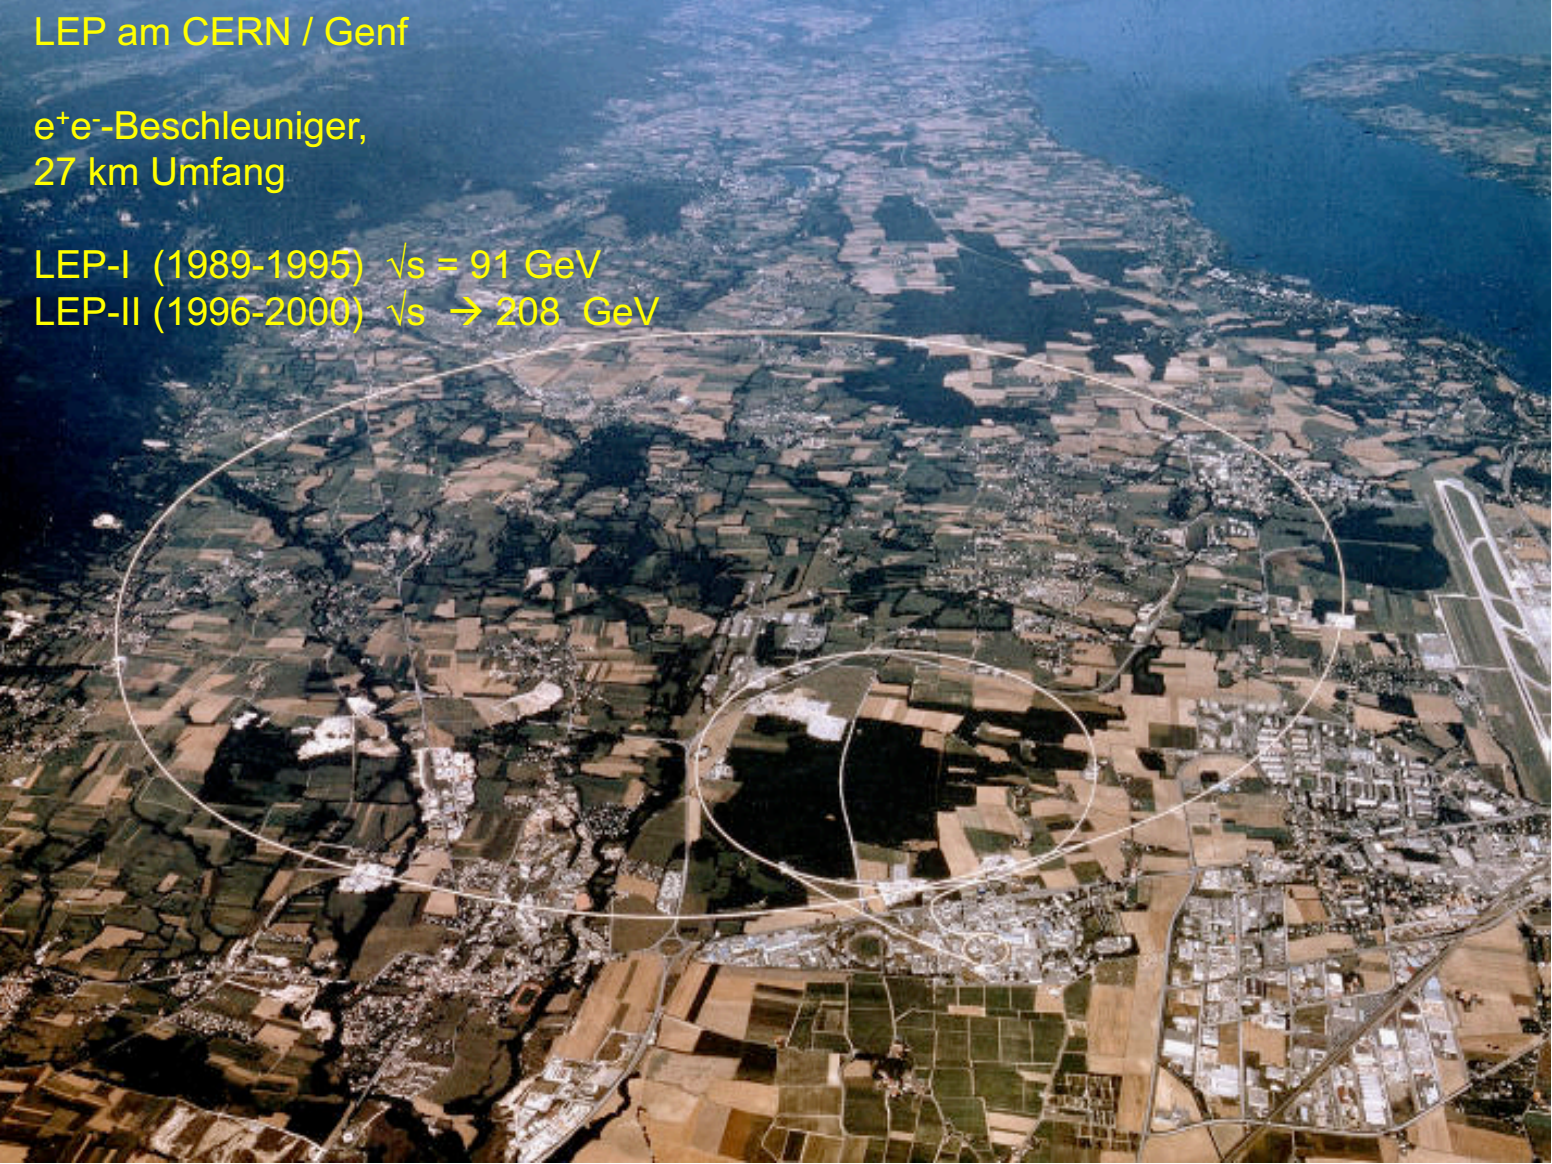
\includegraphics[width=1.0\linewidth]{graphics/LEPmap}
	\end{figure}
\end{frame}

\subsection{Der OPAL Detektor}
\begin{frame}
	\frametitle{Schematischer Aufbau}
	\begin{center}
	\begin{figure}
		\includegraphics[width=0.7\linewidth]{graphics/OPALaufbau}
	\end{figure}
	\end{center}
\end{frame}

\begin{frame}
	\frametitle{Driftkammer}
	\begin{center}
		\begin{figure}
			\includegraphics[width=0.75\linewidth]{graphics/slice_tracking_tr}
		\end{figure}
	\end{center}
	\textbf{Violett:} Vertex Detektor, bestimmt Ereignisort präzise\\
	\textbf{Rot:} Driftkammer, Spuren geladener Teilchen messbar durch Gasentladung
\end{frame}

\begin{frame}
	\frametitle{Elektromagnetisches und hadronisches Kalorimeter}
	\begin{center}
		\begin{figure}
			\includegraphics[width=0.75\linewidth]{graphics/slice_calorimeter_tr}
		\end{figure}
	\end{center}
	\textbf{Türkis: } EM Kalorimeter\\
	\textbf{Gelb: } Hadronisches Kalorimeter
\end{frame}
\begin{frame}
	\frametitle{Schauerbildung}
	\begin{figure}
		\centering
		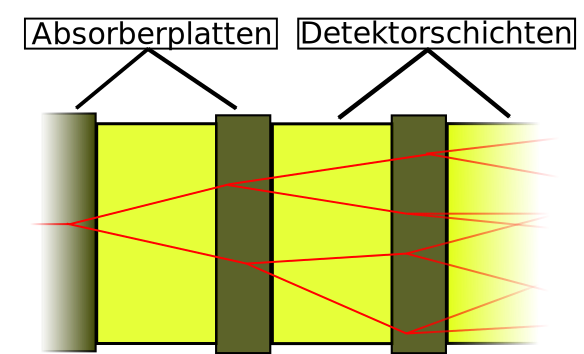
\includegraphics[width=0.7\linewidth]{graphics/Kalorimeter}
	\end{figure}
	\begin{itemize}
		\item Schauerbildung in Absorberblöcken
		\item Energiemessung in Detektorschichten
	\end{itemize}
\end{frame}
\begin{frame}
	\frametitle{Myonenkammer}
	\begin{center}
		\begin{figure}
			\includegraphics[width=0.75\linewidth]{graphics/slice_muon_tr}
		\end{figure}
	\end{center}
\end{frame}




\section{Datenanalyse}
\subsection{Detektor Bilder}
\begin{frame}
	\frametitle{Elektronen Events}
	
\end{frame}

\begin{frame}
	\frametitle{Myonen Events}
	
\end{frame}
\begin{frame}
	\frametitle{Tauonen Events}
	
\end{frame}
\begin{frame}
	\frametitle{Quark Events}
	
\end{frame}
\subsection{Daten der Monte-Carlo Simulation}
\begin{frame}
	\frametitle{Detektorsimulation}
	
\end{frame}
\subsection{Cuts und Aufbereitung der Daten}
\begin{frame}
	\frametitle{E\_Ecal Histogramm}
	
\end{frame}

\begin{frame}
	\frametitle{Zwei Photon Untergrund}
	
\end{frame}

\begin{frame}
	\frametitle{Reinheit der Cuts}
	
\end{frame}
\begin{frame}
	\frametitle{Die Effizienzmatrix}
	
\end{frame}
\begin{frame}
	\frametitle{Die Inverse Effizienzmatrix}
	
\end{frame}

\subsection{Auswertung der aufgearbeiteten Daten}
\begin{frame}
	\frametitle{Wirkungsquerschnitte}

\end{frame}
\begin{frame}
	\frametitle{Masse des $Z^0$ Bosons}
	
\end{frame}
\begin{frame}
	\frametitle{Zerfallsbreiten}
	
\end{frame}
\begin{frame}
	\frametitle{Leptonenuniversalität}
	
\end{frame}
\begin{frame}
	\frametitle{Neutrinogenerationen}
	
\end{frame}
\begin{frame}
	\frametitle{Vorwärts-Rückwärts Asymmetrie}
	
\end{frame}
\begin{frame}
	\frametitle{Berechnung des Weinberg Winkels}
	
\end{frame}







\section{Zusammenfassung und Fehlerdiskussion}
\begin{frame}
	\frametitle{Zusammenfassung}
	
\end{frame}

\AtBeginSection[]{}


\bgroup
\setbeamercolor{background canvas}{bg=black}
\begin{frame}[plain]{}
\end{frame}
\egroup

\end{document}
